%  FICHIER  :   template_fira_two_cols.tex
%  A copier à côté des autres .tex et à déclarer dans config.json
% ------------------------------------------------------------------
\documentclass[11pt,a4paper]{article}

% ─── pack de base ─────────────────────────────────────────────────
\usepackage[T1]{fontenc}
\usepackage[utf8]{inputenc}
\usepackage[british]{babel}
\usepackage[left=0mm,right=0mm,top=0mm,bottom=0mm]{geometry}
\usepackage[stretch=25,shrink=25,tracking=true,letterspace=30]{microtype}
\usepackage{graphicx,xcolor,marvosym,enumitem,paracol,hyperref}
\usepackage{FiraSans}
\renewcommand{\familydefault}{\sfdefault}
\usepackage{array} 
\usepackage{tabularx}
\usepackage{ragged2e}
 \usepackage{fontawesome}
% ─── couleurs & listes ────────────────────────────────────────────
\definecolor{cvblue}{HTML}{304263}
\setlist{parsep=0pt,topsep=0pt,partopsep=1pt,itemsep=1pt,leftmargin=6mm}
\hypersetup{colorlinks=true,urlcolor=white,linkcolor=white}

% ─── macros maison (identiques au modèle original) ────────────────
\newcommand{\dates}[1]{\hfill\textbf{#1}}
\newcommand{\is}{\par\vskip.5ex plus .4ex}
\newcommand{\smaller}[1]{{\small$\diamond$\ #1}}
\newcommand{\headleft}[1]{\vspace*{3ex}\textsc{\textbf{#1}}\par%
  \vspace*{-1.5ex}\hrulefill\par\vspace*{0.7ex}}
\newcommand{\headright}[1]{\vspace*{2.5ex}\textsc{\Large\color{cvblue}#1}\par%
  \vspace*{-2ex}{\color{cvblue}\hrulefill}\par}

% ─── défaut de secours si sidetext absent dans d’autres modèles ───
\providecolor{sidetext}{rgb}{0,0,0}
\definecolor{maincolor}{HTML}{ffffff}
% ─────────────────────────── DOCUMENT ─────────────────────────────
\begin{document}
\thispagestyle{empty}
\setlength{\topskip}{0pt}\setlength{\parindent}{0pt}\setlength{\parskip}{0pt}
\raggedbottom

\begin{minipage}[t]{0.33\textwidth}
  % Bande bleue d’en-tête
  \colorbox{cvblue}{\begin{minipage}[t][5mm][t]{\textwidth}\null\end{minipage}}
  \vspace{-.2ex}
  \colorbox{cvblue!90}{%
    \color{white}\kern0.09\textwidth
    \begin{minipage}[t][293mm][t]{0.82\textwidth}\raggedright
      \vspace*{2.5ex}
      % -------- Identité ------------------------------------------
      \Large Judikael Mourouvin\normalsize

      % Photo (s’affiche seulement si 961c37c0105147ad942478e673381f3c.png ≠ vide)
      \ifx\relax961c37c0105147ad942478e673381f3c.png\relax\else
        \vspace{2ex}\null\hfill
        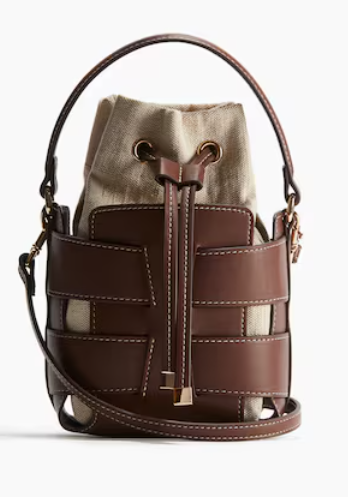
\includegraphics[width=0.65\textwidth]{961c37c0105147ad942478e673381f3c.png}
        \hfill\null
      \fi

      % -------- Profil -------------------------------------------
      \headleft{Profile Summary}
      Technicien informatique passionné par le marketing digital, je dispose d’une solide expérience en support utilisateur, maintenance et gestion de projets numériques. Mon alternance à la DSI de la Mairie du Gosier m’a permis d’affiner mes compétences en analyse des besoins et en déploiement de solutions adaptées. Rigoureux, réactif et orienté satisfaction client, je souhaite désormais poursuivre à plein temps pour optimiser vos systèmes d’information et renforcer votre présence digitale.

      % -------- Contact ------------------------------------------
      \headleft{Contact details}\small
      \MVAt\  \texttt{jkmou971@gmail.com}\par
      \Mobilefone\ +590 690 91 14 48\par
      \Letter\ Route de Cocoyer\par
      97190 Gosier\par
      \faLinkedin\  \href{}{}
      \normalsize

      % -------- Langues (si dispo) -------------------------------
      \ifx\relax\begin{itemize}[leftmargin=*]
\item Anglais - \textcolor{gray}{}
\item Espagnol - \textcolor{gray}{}\end{itemize}\relax\else
        \headleft{Languages}
        \begin{itemize}[leftmargin=*]
\item Anglais - \textcolor{gray}{}
\item Espagnol - \textcolor{gray}{}\end{itemize}
      \fi

      % -------- Compétences --------------------------------------
      \headleft{Skills}
      \begin{itemize}[leftmargin=*]
\item Réseaux
\item Support
\item Maintenance
\item Configuration
\item Marketing
\item Digital
\item Assistance\end{itemize}

      % -------- Centres d’intérêt --------------------------------
      \headleft{Hobbies}
      \begin{itemize}[leftmargin=*]
\item Lecture \& veille technologique
\item Randonnée / sports outdoor
\item Voyages \& découverte culturelle
\end{itemize}

    \end{minipage}\kern0.09\textwidth
  }
\end{minipage}
% ================================================================
\hskip2.5em
% ======================= COLONNE DROITE =========================
\begin{minipage}[t]{0.56\textwidth}
  \setlength{\parskip}{0.8ex}
  \vspace{2ex}

  % ---------- EXPERIENCE ----------------------------------------
  \headright{Experience}
  
\colorbox{maincolor}{%
  \begin{minipage}{\linewidth}
    \textbf{Alternant en marketing digital} \\ Mairie du Gosier – DSI \\ 2023-2024
    \begin{itemize}
      \item Piloté des projets numériques pour la DSI, garantissant leur déploiement dans les délais. \item Analysé les besoins des agents et implémenté des solutions adaptées, améliorant l’efficacité opérationnelle. \item Assuré support et formation des utilisateurs, facilitant l’adoption des outils de marketing digital.
    \end{itemize}
  \end{minipage}}

\vspace{3mm}


\colorbox{maincolor}{%
  \begin{minipage}{\linewidth}
    \textbf{Animateur de la zone informatique} \\ Pôle Emploi, Gosier \\ 2022-2023
    \begin{itemize}
      \item Accueilli et assisté les usagers sur l’espace informatique, résolvant leurs problématiques techniques. \item Configuré et entretenu les postes de travail afin de garantir un environnement fiable. \item Diagnostiqué et corrigé les incidents, limitant les interruptions de service.
    \end{itemize}
  \end{minipage}}

\vspace{3mm}


\colorbox{maincolor}{%
  \begin{minipage}{\linewidth}
    \textbf{Stagiaire informaticien} \\ Numerika, Baie-Mahault \\ 2020-2021
    \begin{itemize}
      \item Installé et paramétré les équipements informatiques, assurant leur fonctionnement optimal. \item Fournit un support de proximité aux utilisateurs, améliorant leur autonomie. \item Effectué la maintenance préventive du parc, prolongeant la durée de vie du matériel.
    \end{itemize}
  \end{minipage}}        % ← déjà formaté par build_placeholders()

  % ---------- EDUCATION -----------------------------------------
  \headright{Education}
  
    \begin{tabularx}{\linewidth}{@{}c >{\RaggedRight\arraybackslash}X@{}}
    \textcolor{sidetext}{\faGraduationCap} &
    \textbf{Bachelor Marketing Digital} \\
    & CFA IUTS \\
    & \textit{2023-2024} \\
    \end{tabularx}
    \begin{itemize}[leftmargin=*]
  \item Acquisition des fondamentaux du référencement, des réseaux sociaux et de l’analyse de données.
  \item Conduite de projets web et campagnes marketing multicanal.
  \item Développement de compétences en gestion de contenu et veille digitale.
\end{itemize}
\vspace{3mm}

    \begin{tabularx}{\linewidth}{@{}c >{\RaggedRight\arraybackslash}X@{}}
    \textcolor{sidetext}{\faGraduationCap} &
    \textbf{BTS Système Numérique option Informatique et Réseaux} \\
    & Lycée de Chevalier Saint-Georges, Abymes \\
    & \textit{2019-2021} \\
    \end{tabularx}
    \begin{itemize}[leftmargin=*]
  \item Étude des architectures réseau, des protocoles et de la cybersécurité.
  \item Pratique de l’installation, de la maintenance et du diagnostic matériel/logiciel.
  \item Réalisation de projets d’intégration et d’assistance technique.
\end{itemize}

\end{minipage}

\end{document}
